% !TEX root =  ../report.tex

\section{Introduction}
%The introduction should provide content for the report, discuss relevant background material and state the main aims of the work. Clearly establishing the aims of the work is important for this coursework, since you have a great deal of freedom in what you will seek to achieve.

In the field of High Performance Computing (HPC), computers with processing power hundreds of times greater than conventially available machines are used to solve or approximate complex problems. Such computers have been required for some time to utilise parallelism, in order to find solutions within a reasonable run-time.
\par Many paradigms for executing parallel workloads have emerged over time. Recently, General Purpose Graphical Processing Units (GPGPUs) have become an increasingly popular hardware architecture, having originally been concieved as specilised hardware for graphical shader calculations. GPU's high number of parallel processing units allow a high degree of parallelism, as well as being able to execute operations usually done by the CPU. Passing work to the GPU device can provide very significant speed-up over sequential execution.
\par
Commonly, a single developer or team is unlikely to have both the necessary expertise in both a niche area of physics with a non-trivial problem to be solved; and also sufficient depth of knowledge in computer science to understand the latest generation of parallel hardware. For this reason the OP2 framework was created: to provide a high level abstraction in which HPC applications can be written, and seperate the application code from the optimisation requirements. OP2 already is able to generate optimised code for a number of backends from an application file.
\par
This report details an investigation into applying a new optimisation to the CUDA code generation in OP2, and the process of benchmarking what performance gain, if any, it is able to provide.
The optimisation is named``Just-In-Time Compilation" for its similarities to a comparable process often performed by compilers when run-time efficiency is desired.
\vfill
\subsection{Motivations}
The idea for this project was provided by my supervisor, Dr Gihan Mudalige - an Associate Proffesor in the University of Warwick Computer Science Department. It was pulled from the pool of uncompleted features for the OP2 project, and was selected because it aligned with my interest in High Performance Computing, and previous experience with optimising exisiting codes.
\par
Since OP2 is Open Source and freely available, the implementation I produce will become part of the library, allowing future contributors to build on my work.

\subsection{Background Work}
\label{s:bgwork}

In order to become comfortable with the OP2 framework, and provide a useful contribution, it is important to understand the domain of problems for which it was created: Unstructured Mesh Solvers.
\par
A large proportion of HPC workloads involve approximating Partial Differential Equations (PDEs) to simulate complex interactions in physics problems, for example the Navier-Stokes equations for computational fluid dynamics, or prediciting weather patterns. It is usually necessary to discretise such problems, dividing 2D or 3D space into a number of cells. Depending on its structure this mesh can be described as either structured (regular) or unstructured.

\begin{figure}[h!]
  \begin{minipage}{.5\textwidth}
    \centering
    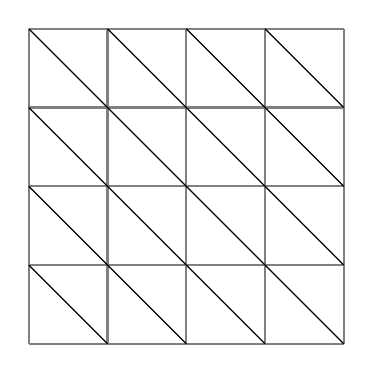
\begin{tikzpicture}
      \draw[step=1cm,gray,thick]
      (0,0) grid (4,4);

      \foreach \x in {0,...,3}{
        \draw (\x, 0) -- (0, \x) ;
        \draw (\x, 4) -- (4, \x) ;
      }

    \end{tikzpicture}
    \caption{Tri-Structured Mesh}
    \label{fig:struct}
  \end{minipage}
  \begin{minipage}{.5\textwidth}
    \centering
    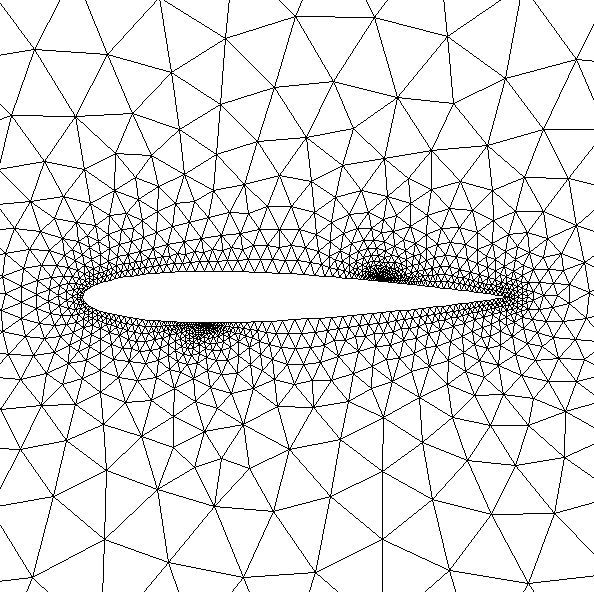
\includegraphics[width=.55\textwidth]{umesh}
    \caption{Airfoil Tri-Unstructed Mesh}
    \label{fig:umesh}
  \end{minipage}
\end{figure}
Unstructed Meshes, such as Figure \ref{fig:umesh}, use connectivity information to specify the mesh topology. The position of elements is highly arbritrary, unlike structured meshes where elements follow a regular pattern (Figure \ref{fig:struct}). A particular simulation might, for example, be approximating the velocity of a fluid in each cell, and at every time step re-calculating this value based on the values of cells around it.
\par
Since a structured mesh can be represented using an unstructured mesh, OP2 can support either - however unstructured meshes are more common.

\subsection{Report Structure}
The rest of this report is structured as follows: In Section \ref{s:research} (p\pageref{s:research}) the research done to inform the work in this project is discussed, followed by a Specification in Section \ref{s:spec} (p\pageref{s:spec}).
Section \ref{s:impl} (p\pageref{s:impl}) details the Implemention and expected results, Section \ref{s:test} (p\pageref{s:test}) explains the Testing and Benchmarking of the project, and Section \ref{s:eval} (p\pageref{s:eval}) an Evaluation of the work completed, including Project Management (p\pageref{ss:pm}).
 Lastly, Section \ref{s:fw} (p\pageref{s:fw}) contains a discussion on Future Work which could build on top of what was done for this report, and Section \ref{s:conc} (p\pageref{s:conc}) an overall Conclusion
